\documentclass[12pt, letterpaper]{article}
\usepackage[utf8]{inputenc}
\usepackage{graphicx}
\graphicspath{ {./images/} }
\title{\textbf{Srilankan Economic Crisis}}
\author{\textit{Ahmed Reza Riday} }
\date{May 22}\documentclass{article}
\begin{document}
\begin{titlepage}
\maketitle
\begin{figure}[b]
\fromsig{
\includegraphics[scale=1]{p}}

\thanks{Ahmed Reza Riday}
\end{figure}
\end{titlepage}

\begin{enumerate}
\LARGE
  \item Introduction.
  \item Economic Fall. 
  \item Learning For Bangladesh.
\end{enumerate}
\newpage{
\begin{enumerate}
\LARGE
  \item \underline{Introduction:}
  \large{The 2019–2022 Sri Lankan economic crisis, currently affecting the island nation of Sri Lanka, is largely attributed to economic mismanagement by its incumbent government.}
\end{enumerate}
\begin{enumerate}
\LARGE
  \item \underline{Economic Fall:}
  \large{In 2021, the Sri Lankan Government officially declared the worst economic crisis in the country in 73 years. In August 2021, a food emergency was declared. However the government denied food shortages. Sri Lanka's Energy Minister Udaya Gammanpila acknowledged the crisis could lead to a financial disaster.}
\end{enumerate}
\begin{enumerate}
\LARGE
  \item \underline{Learning For Bangladesh:}
  \large{Despite repeated warnings from economists, Bangladesh so far hasn't taken any major stride toward diversification of its export basket. It still depends heavily on the garment sector.

The economic crisis in Sri Lanka caused by factors including a slump in foreign currency flow from two main sources -- tourism and remittances --- once again gives a reminder that diversification is a necessity, not an option.}
\end{enumerate}
}
\newpage{
\begin{equation} \label{eq1}
\begin{split}
Principal Repayment & = \frac{\frac{r}{n} * (1+\frac{r}{n})^tXn}{(1+\frac{r}{n})^tXn-1} \\
 - \frac{PXr}{n}
\end{split}
\end{equation}
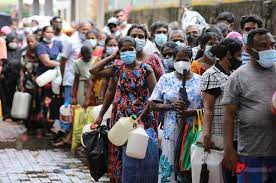
\includegraphics{rr}
Srilankan Economic Crisis
\begin{center}
\begin{tabular}{||c c c c||} 
 \hline
 Year & GDP & PCI & Loan \\ [0.5ex] 
 \hline\hline
 2018 & 87.95 & 4059 &  \\ 
 \hline
 2019 & 83.98 & 3,851.67 &  \\
 \hline
 2020 & 80.71 & 3,679 &  \\
 \hline
 2021 & 81 & 4100 &  \\
 \hline
 2022 & 83 & 4300 &  \\ [1ex] 
 \hline
\end{tabular}
\end{center}
}



\end{document}
